

\documentclass{article}

\usepackage[utf8]{inputenc}

\usepackage{fullpage} % Package to use full page
\usepackage{parskip} % Package to tweak paragraph skipping
\usepackage{tikz} % Package for drawing
\usepackage{amsmath}
\usepackage{hyperref}
\usepackage{bm}
\usepackage{appendix}
\usepackage{graphicx}
\usepackage[caption=false]{subfig}
\usepackage{float}
\usepackage{enumitem}
\usepackage{algorithm}
\usepackage{algpseudocode}


\title{ITR Project Version 2.0 : comprehensive search implementation}

\author{Jie Xue}


\date{\today}
\begin{document}
\maketitle
\tableofcontents
\pagebreak


\section{Introduction}
\subsection{Individual treatment recommendation}
According to Wiki, precision medicine is a medical model that proposes the customization of healthcare, with medical decisions, practices, and/or products being
tailored to the individual patient. In this model, diagnostic testing is often
employed for selecting appropriate and optimal therapies based on the
context of a patient's genetic content or other molecular or cellular
analysis. Tools employed in precision medicine can include molecular
diagnostics, imaging, and analytics/software.

With new treatments and novel technology available, personalized medicine has become an important piece in the
new era of medical product development. Traditional statistics methods for personalized medicine and subgroup
identification primarily focus on single treatment or two arm randomized control trials. Motivated by the recent
development of outcome weighted learning framework, we propose an alternative algorithm to search treatment
assignments which has a connection with subgroup identification problems. Our method focuses on applications
from clinical trials to generate easy to interpret results. This framework is able to handle two or more than two
treatments from both randomized control trials and observational studies. We implement our algorithm in C++. 

\subsection{Mathematical background}
\begin{itemize}
\item There are $N$ subjects from a large population.
\item $A_i$ is the treatment assignment (actions), where $i = 1,\ldots,N$.
\item $Y_i$ is the response assuming that larger $Y_i$ is better (rewards).
\item $X_i$ is a vector of covariates.
\item $\left(Y , A, X\right)$ is the generic random variable of $\{\left(Y_i , A_i, X_i\right)\}$.
\item $\mathcal{P}$ is the distribution of $\left(Y , A, X\right)$.
\item $E$ is the expectation with respect to $\mathcal{P}$.
\item Population space $\chi$, i.e. ${X _i} \in \chi$
\item $\mathcal{D}\left(\cdot\right)$ is a treatment recommendation based on covariates, i.e.
$\mathcal{D}\left(\cdot\right) : \chi  \to A$.
\item $\mathcal{P^D}$ is the distribution of $\left(Y , A, X\right)$ given that $A = \mathcal{D}\left( X \right)$.
\end{itemize}

Define
\[{E^\mathcal{D}}\left( Y \right) = \int {Yd{\mathcal{P^D}}}  = \int {Y\frac{{d\mathcal{P^D}}}{{d\mathcal{P}}}d\mathcal{P} = E\left[ {\frac{{I\left\{ {A = \mathcal{D}\left( X \right)} \right\}}}{{p\left( {A|X} \right)}}Y} \right]} \]
where
\[\frac{{d\mathcal{P^D}}}{{d\mathcal{P}}} = \frac{{p\left( {y|x,a} \right)I\left\{ {a = \mathcal{D}\left( x \right)} \right\}p\left( x \right)}}{{p\left( {y|x,a} \right)p\left( {a|x} \right)p\left( x \right)}} = \frac{{I\left\{ {a = \mathcal{D}\left( x \right)} \right\}}}{{p\left( {a|x} \right)}}\]

Our objective is to find $\mathcal{D}\left(\cdot\right)$ to maximize the following value function:
\[{\mathcal{D}_o} \in \mathop {\arg \max }\limits_{\mathcal{D} \in R} {E^\mathcal{D}}\left( Y \right) = E\left[ {\frac{{I\left\{ {A = \mathcal{D}\left( X \right)} \right\}}}{{p\left( {A|X} \right)}}Y} \right]\]
where $R$ is a space of possible treatment recommendations.

Example 1 depth search (from ITR.ABC):

Suppose we have two doctors and each of them has a treatment rule.
Which doctor is a better one?
\begin{itemize}
\item Doctor Adam: give patients treatment 1 if $X \geq 2$, and treatment 2 otherwise, denoted as $\mathcal{D}_A\left(X\right)$.
\item Doctor Barry: give patients treatment 1 if $X \geq 3$, and treatment 2 otherwise, denoted as $\mathcal{D}_B\left(X\right)$.
\end{itemize}

\begin{table}[H]
\centering
\caption{Example calculation}
\begin{tabular}{c|ccc|ccccc}
\hline \hline
ID & $Y$ & $A$ & $X$ & $P\left( {A|X} \right)$ & $\mathcal{D}_A$ & $\mathcal{D}_B$ & $\mathcal{D}_A = A$ & $\mathcal{D}_B = A$ \\ \hline
1  & 1 & 1 & 1 & 0.5    & 2  & 2  & 0   & 0   \\
2  & 2 & 1 & 2 & 0.5    & 1  & 2  & 1   & 0   \\
3  & 3 & 1 & 3 & 0.5    & 1  & 1  & 1   & 1   \\
4  & 4 & 1 & 4 & 0.5    & 1  & 1  & 1   & 1   \\
5  & 5 & 1 & 5 & 0.5    & 2  & 2  & 1   & 1   \\
6  & 3 & 2 & 1 & 0.5    & 1  & 2  & 1   & 1   \\
7  & 3 & 2 & 2 & 0.5    & 1  & 1  & 0   & 1   \\
8  & 3 & 2 & 3 & 0.5    & 1  & 1  & 0   & 0   \\
9  & 3 & 2 & 4 & 0.5    & 1  & 1  & 0   & 0   \\
10 & 3 & 2 & 5 & 0.5    & 1  & 1  & 0   & 0   \\ \hline \hline
\end{tabular}
\end{table}

Doctor Adam:
\[
\begin{aligned}
{E^{{\mathcal{D}_A}}}\left( Y \right) &= \frac{1}{{10}}\left( {\frac{0}{{0.5}} \times 1 + \frac{1}{{0.5}} \times 2 + \frac{1}{{0.5}} \times 3 + \frac{1}{{0.5}} \times 4 + \frac{1}{{0.5}} \times 5 + \frac{1}{{0.5}} \times 3 + \frac{0}{{0.5}} \times 3 + \frac{0}{{0.5}} \times 3 + \frac{0}{{0.5}} \times 3 + \frac{0}{{0.5}} \times 3} \right)\\ 
 &= 3.4
\end{aligned}
\]

Doctor Barry:
\[
\begin{aligned}
{E^{{\mathcal{D}_B}}}\left( Y \right) &= \frac{1}{{10}}\left( {\frac{0}{{0.5}} \times 1 + \frac{0}{{0.5}} \times 2 + \frac{1}{{0.5}} \times 3 + \frac{1}{{0.5}} \times 4 + \frac{1}{{0.5}} \times 5 + \frac{1}{{0.5}} \times 3 + \frac{1}{{0.5}} \times 3 + \frac{0}{{0.5}} \times 3 + \frac{0}{{0.5}} \times 3 + \frac{0}{{0.5}} \times 3} \right)\\ 
 &= 3.6
\end{aligned}
\]

Conclusion: Doctor Barry's rule is better than Doctor Adam's.

\subsection{Logic for comprehensive search}
The comprehensive searching problem could be formulated as nested conditional operations with independent, exclusive mutual criteria.

Assume we have three criteria, $c_1$, $c_2$, and $c_3$. For each criteria, there would be a binary result for satisfied giving 1 or unsatisfied giving 0.
\begin{figure}[H]
\centering
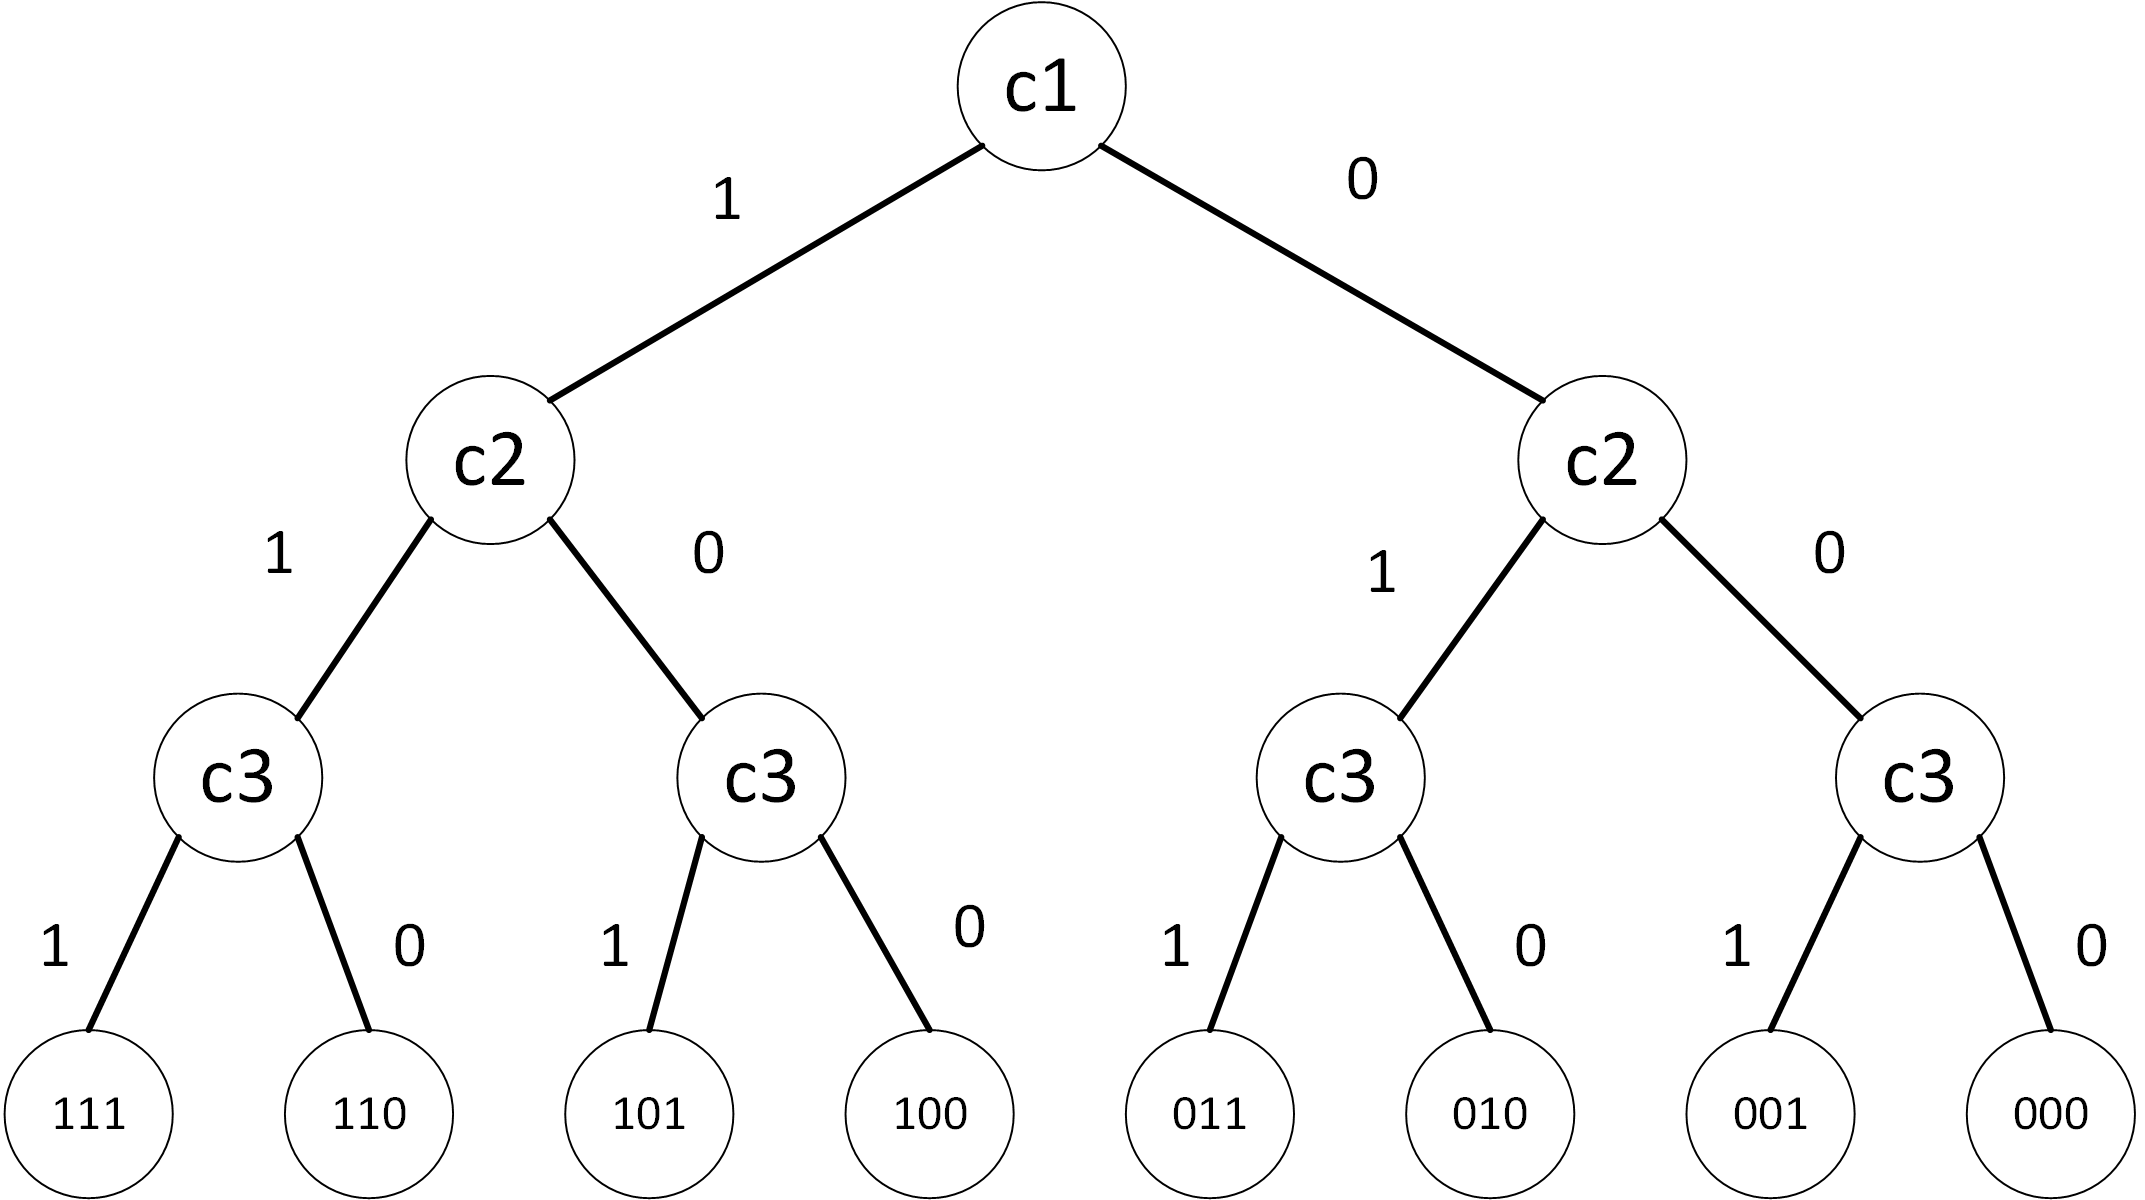
\includegraphics[width=1\textwidth]{ITR_logic.png}
\end{figure}
Therefore, there exists 8 possible results from 111 to 000 which fits a 8 length vector. In this project, the last criteria checks if the patient applies treatment 1. As a result, the expectation for results 1 (11) use the information of 110, 100, 010, and 000. If we know the summation of all response that take treatment 0. Result 1 could be simplified as the function of 111 and 110.


\pagebreak
\section{Architecture and Design}
\subsection{Design goals}
In the project, we implement the ITR comprehensive search by using C++11. Apply appropriate design pattern with the consideration of abstraction, code reuse, stability, and scalability. The desired running time is less than 120s.

\subsection{Class Diagram}
\begin{figure}[H]
\caption{UML class diagram}
\centering
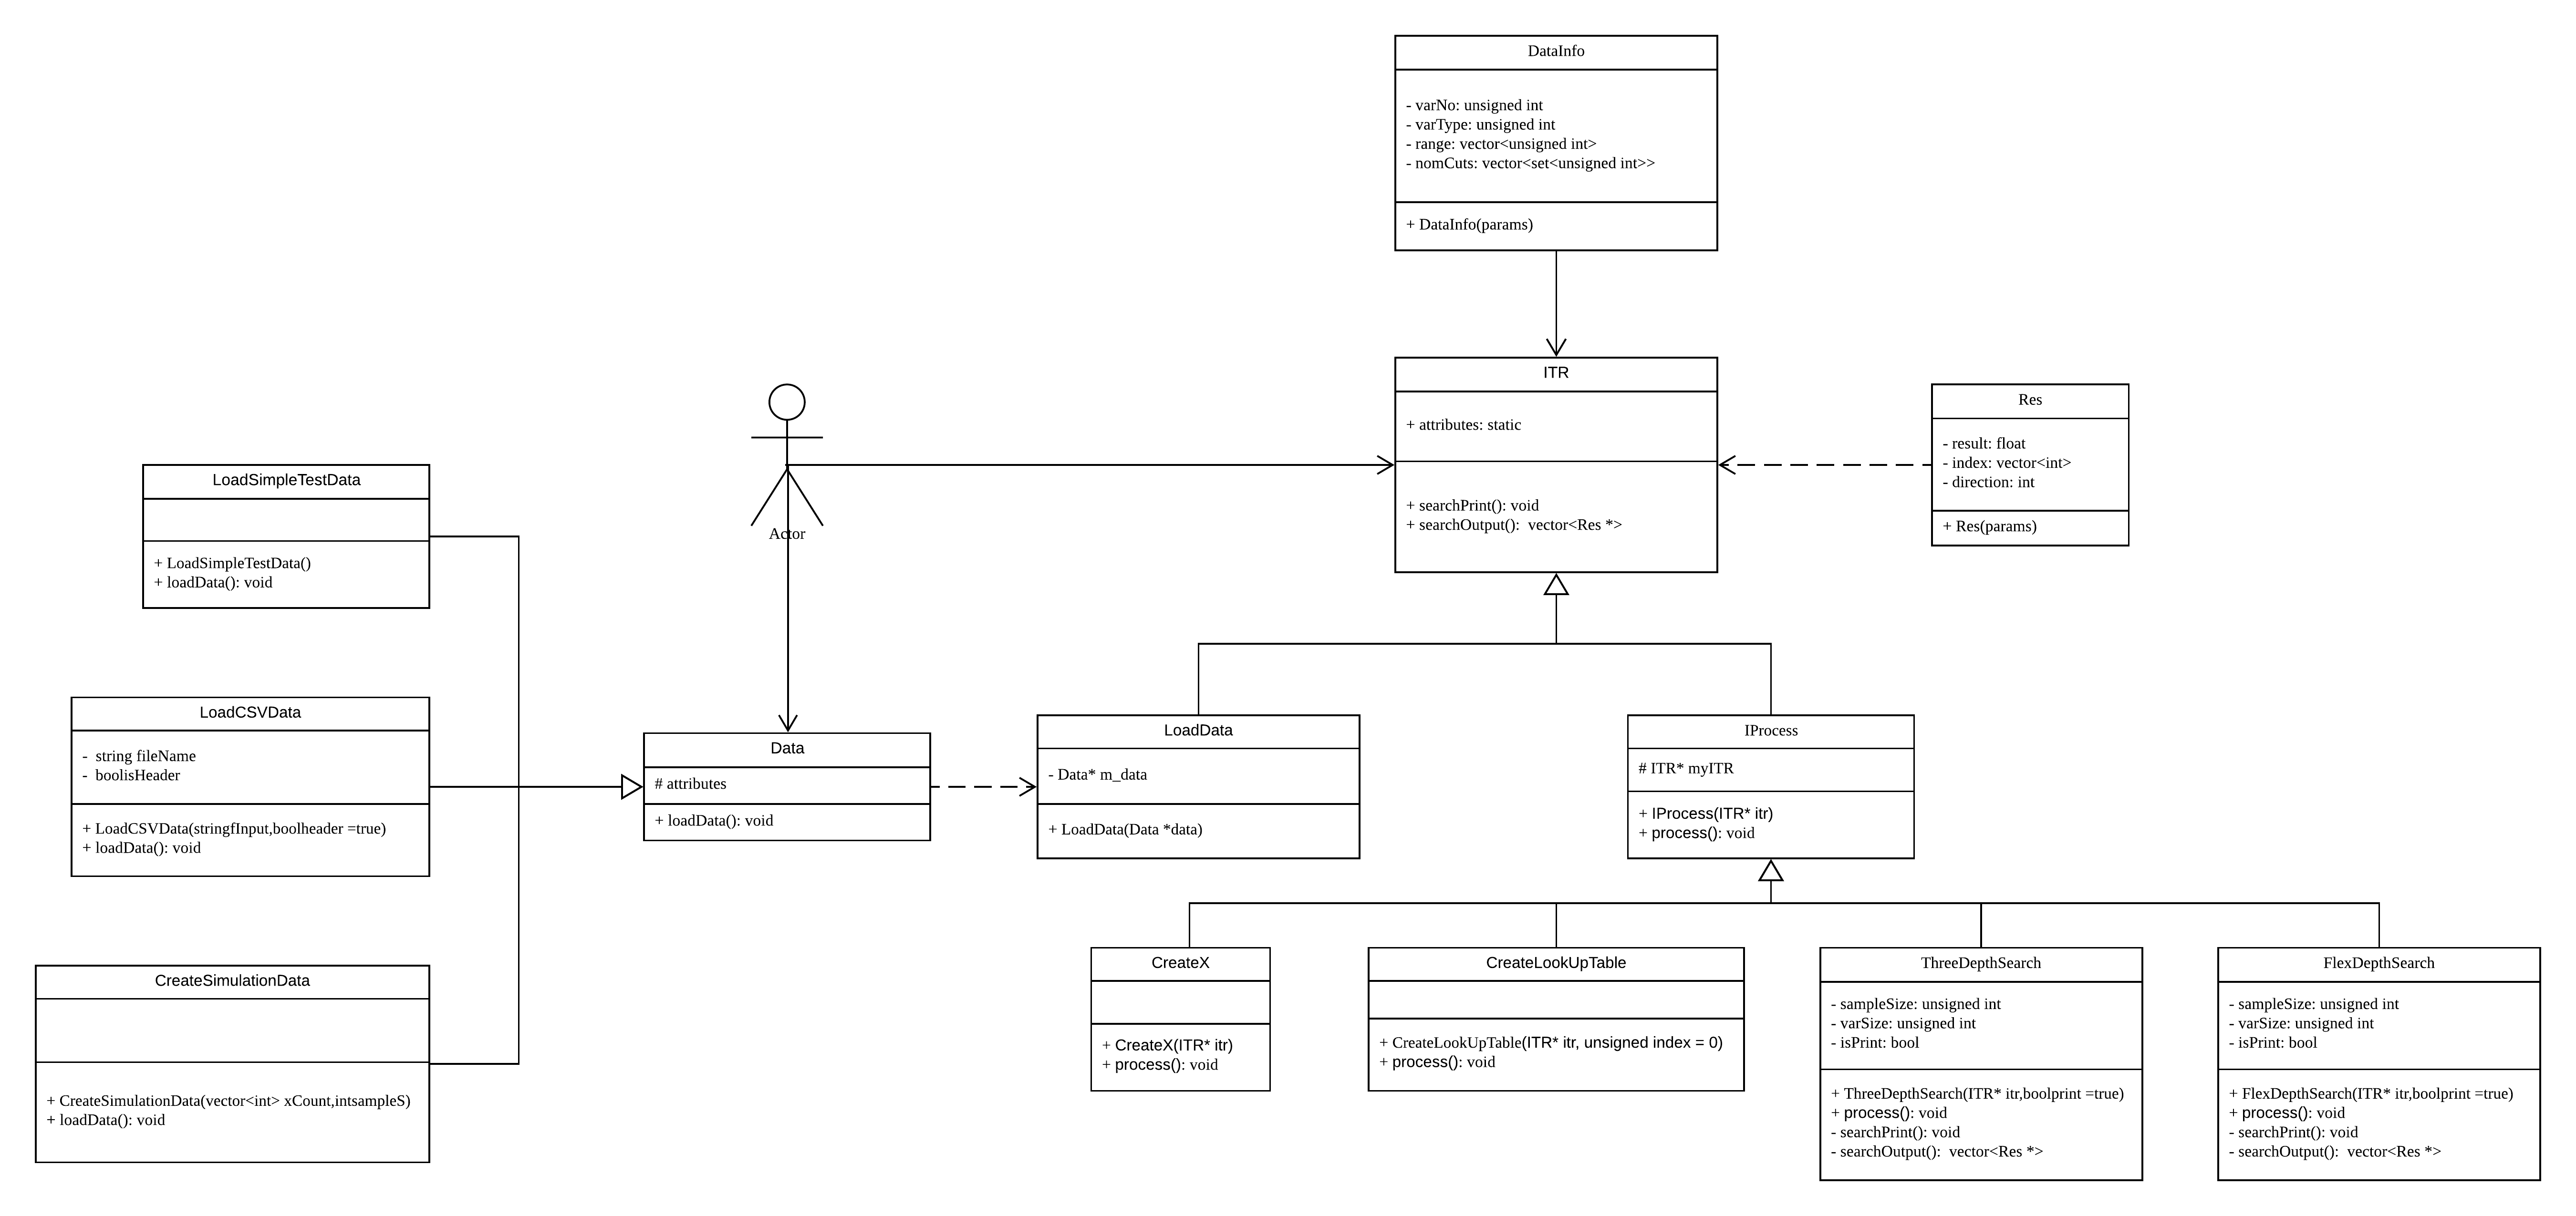
\includegraphics[width=1\textwidth]{UML_Class.png}
\end{figure}

The ITR system is comprised of 4 main parts as following:
\begin{itemize}
\item Res: Store results
\item DataInfo: generate searching information for each variable
\item Data: interface for input data
\begin{itemize}
\item LoadSimpleTestData: load ITR.ABC example data
\item LoadCSVData: load CSV data of 9 covariants, 100 samples
\item CreateSimulationData: create simulation data 
\end{itemize}
\item ITR: class for comprehensive search
\begin{itemize}
\item LoadData: load data (base class for ITR)
\item IProcess: interface for operations
\begin{itemize}
\item[$\circ$] CreateX: merge types of data
\item[$\circ$] CreateLookUpTable: create look up table
\item[$\circ$] OneDepthSearch: 1 depth search
\item[$\circ$] TwoDepthSearch: 2 depth search
\item[$\circ$] ThreeDepthSearch: 3 depth search
\item[$\circ$] FlexDepthSearch: flexible depth search
\end{itemize}

\end{itemize}

\end{itemize}

The decorate method design pattern is applied for Data.

The decorator pattern is implemented for ITR operation.

\subsection{Sequence Diagram}
\begin{figure}[H]
\centering
\caption{UML sequence diagram}
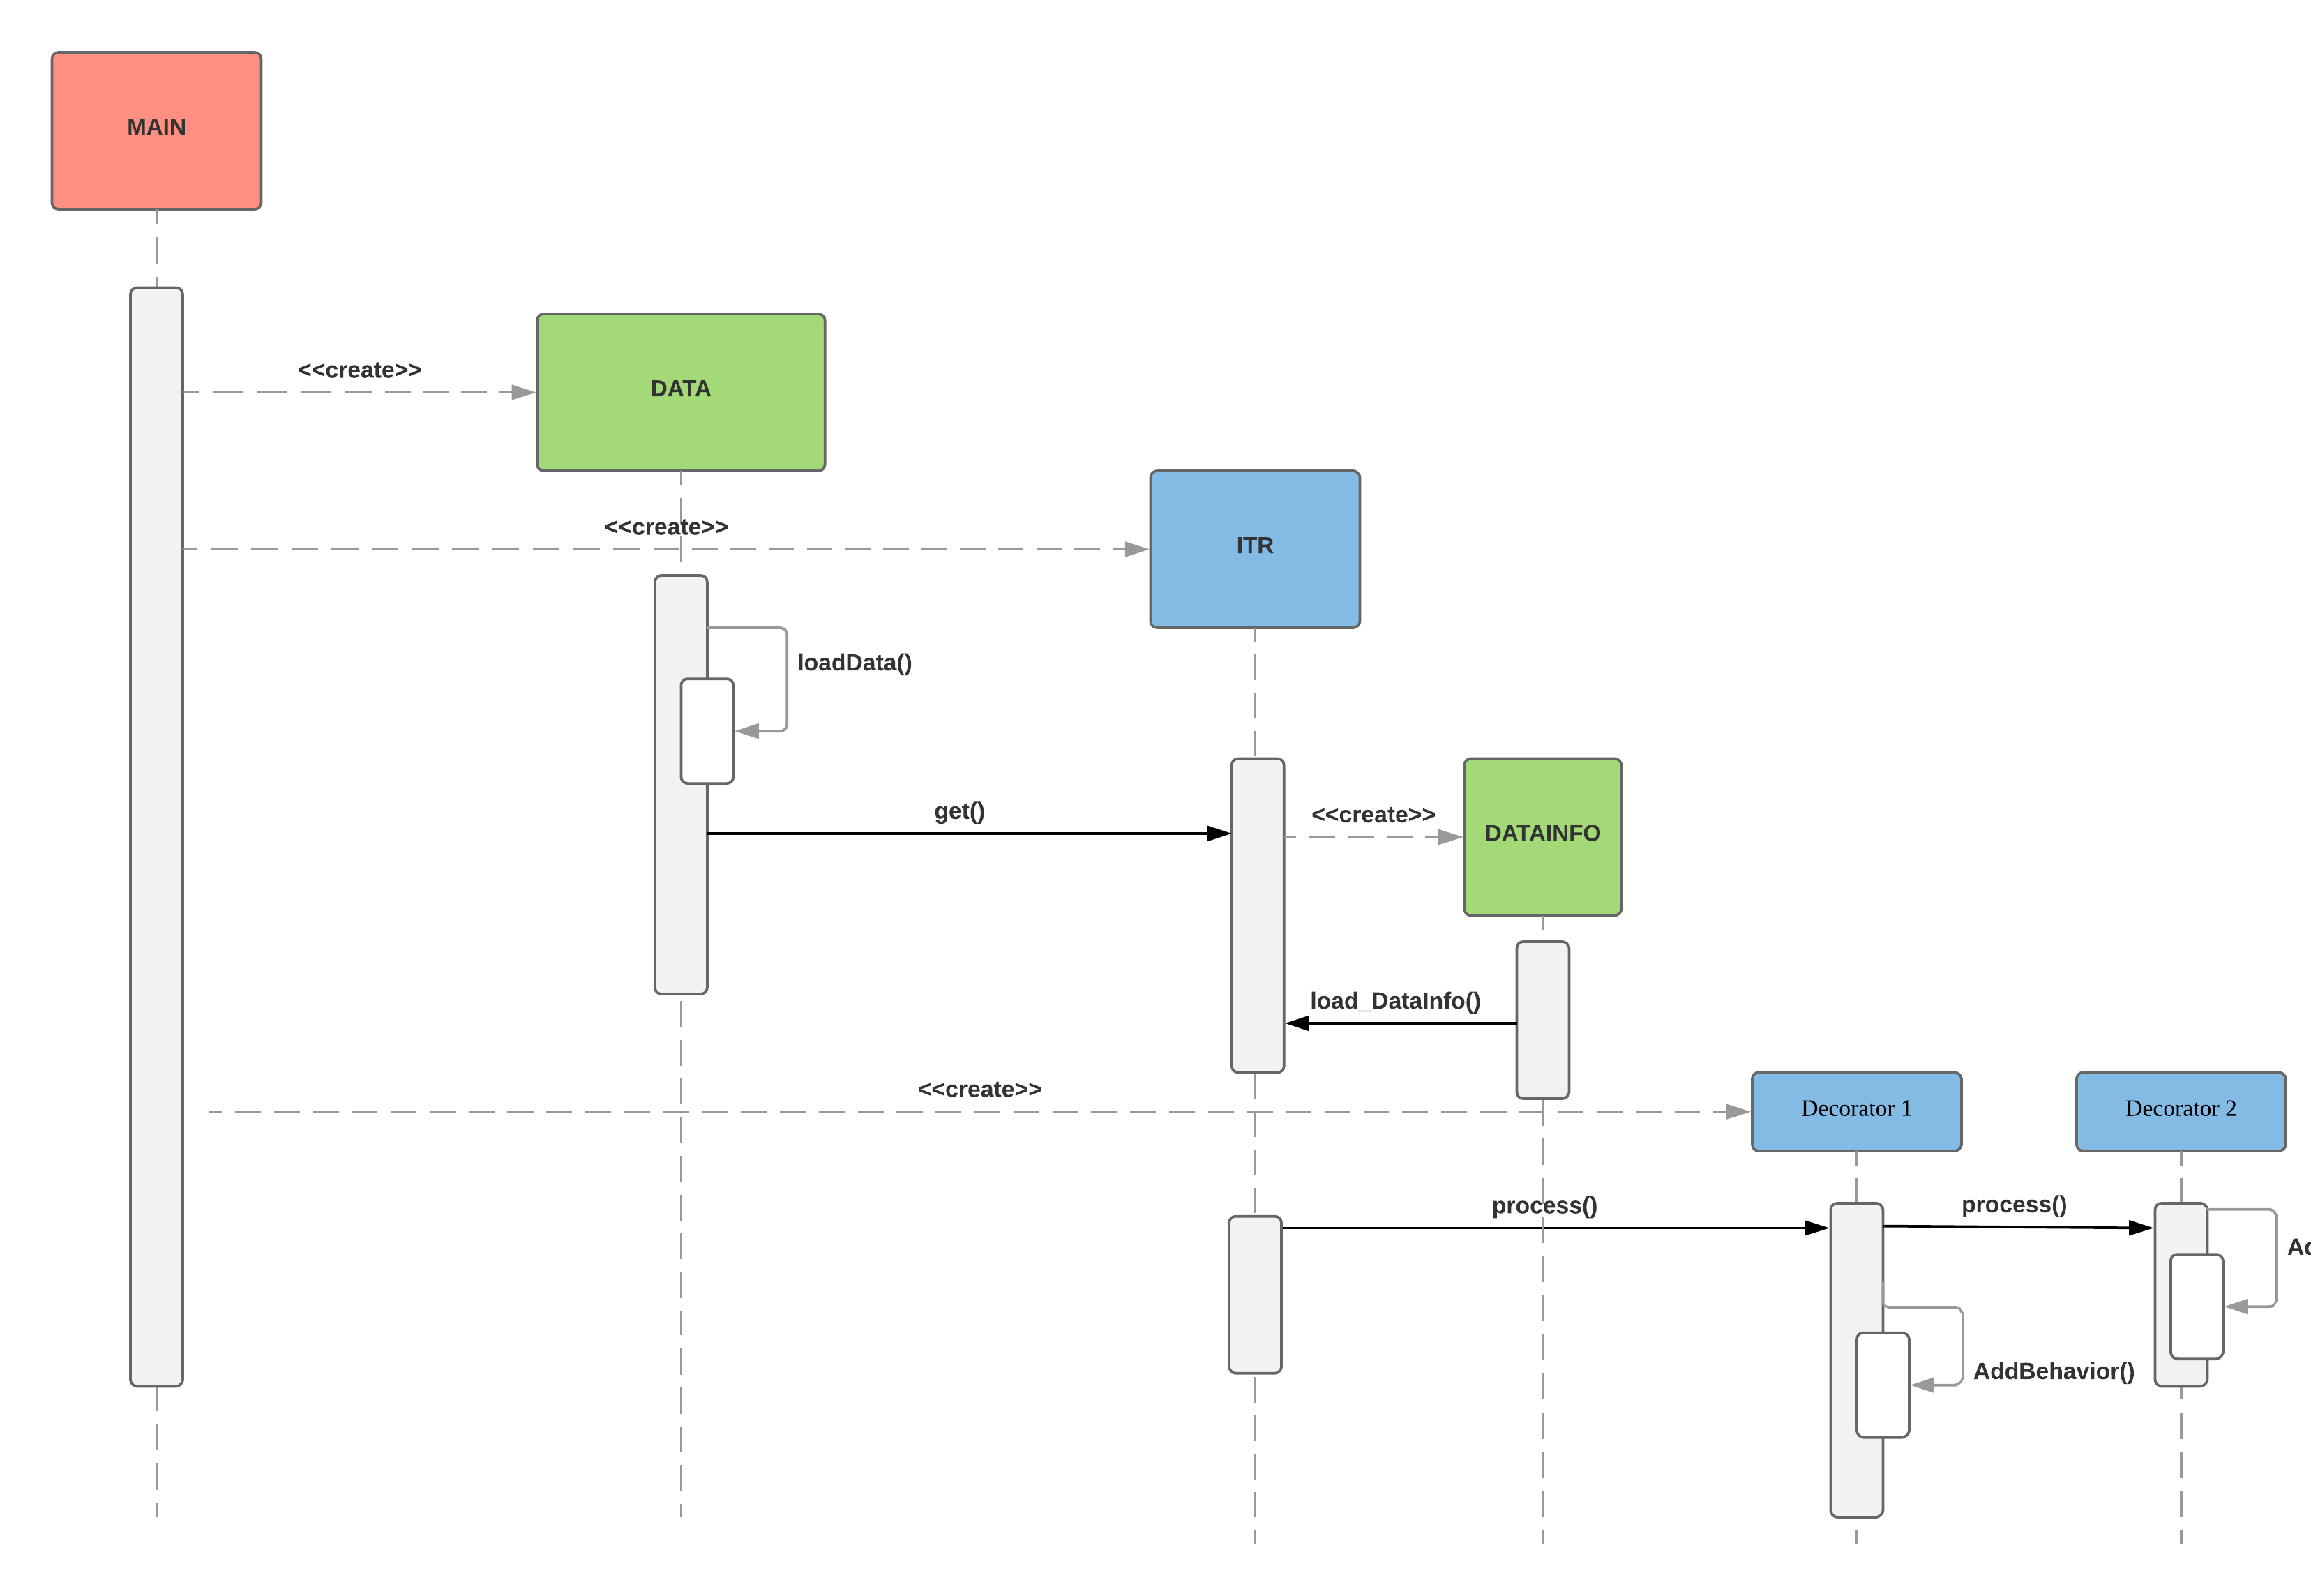
\includegraphics[width=1\textwidth]{UML_Seq.png}
\end{figure}

The data class is first created. Then data is passed to ITR through a pointer. DataInfo is called to generate criteria information for each variable. Decorators could be added depends on the algorithm.



\subsection{Detailed Class Design}
\subsubsection{Data Class Reference}
The purpose of the interface Data is to load or create data.

Inheritance diagram for Data:
\begin{figure}[H]
\centering
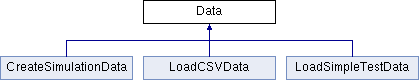
\includegraphics[width=0.8\textwidth]{class_data.png}
\end{figure}

\textbf{Protected Attributes}:
\begin{itemize}
\item unsigned int sampleSize                               
\item vector$<$unsigned int$>$ id                               
\item vector$<$vector$<$double$>>$ y                               
\item vector$<$vector$<$unsigned int$>>$ actions              
\item vector$<$vector$<$double$>>$ x\_Cont;                          
\item vector$<$vector$<$unsigned int$>>$ x\_Ord                  
\item vector$<$vector$<$unsigned int$>>$ x\_Nom                    
\item vector$<$unsigned int$>$ dataType
\end{itemize}

\textbf{Public Member Functions}
\begin{itemize}
\item \textbf{Data}(): constructor
\item virtual void \textbf{loadData}(): virtual function
\item const vector$<$unsigned int$>$\& \textbf{getID}()
\item const vector$<$vector<double$>>$\& \textbf{getY}()
\item const vector$<$vector<unsigned int$>>$\& \textbf{getActions}()
\item const vector$<$vector<double$>>$\& \textbf{getX}\_\textbf{Cont}()
\item const vector$<$vector$<$unsigned int$>>$\& \textbf{getX}\_\textbf{Ord}()
\item const vector$<$vector$<$unsigned int$>>$\& \textbf{getX}\_\textbf{Nom}()
\item const vector$<$unsigned int$>$\& \textbf{getX}\_\textbf{Type}()
\item unsigned int \textbf{getSampleSize}()
\end{itemize}


More information about this class can be found from the following files:
\begin{itemize}
\item Data.h
\item Data.cpp
\end{itemize}

\subsubsection{LoadSimpleTestData Class Reference}
The purpose of LoadSimpleTestData class is load data given by ITR.ABC.

Inheritance diagram for LoadSimpleTestData:
\begin{figure}[H]
\centering
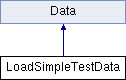
\includegraphics[width=0.2\textwidth]{class_load_simple_test_data.png}
\end{figure}


\textbf{Public Member Functions}
\begin{itemize}
\item \textbf{LoadSimpleTestData}() : constructor
\item void \textbf{loadData}() : overload
\end{itemize}

More information about this class can be found from the following files:
\begin{itemize}
\item LoadSimpleTestData.h
\item LoadSimpleTestData.cpp
\end{itemize}



\subsubsection{LoadCSVData Class Reference}
The purpose of LoadCSVData class is load CSV data.

Inheritance diagram for LoadCSVData:
\begin{figure}[H]
\centering
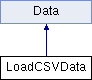
\includegraphics[width=0.2\textwidth]{class_load_c_s_v_data.png}
\end{figure}

\textbf{Private Attributes}:
\begin{itemize}
\item string fileName
\item bool isHeader
\end{itemize}

\textbf{Public Member Functions}:
\begin{itemize}
\item \textbf{LoadCSVData}(string fInput, bool header = true): constructor, default header = true
\item void \textbf{loadData}() : overload
\end{itemize}


More information about this class can be found from the following files:
\begin{itemize}
\item LoadCSVData.h
\item LoadCSVData.cpp
\end{itemize}


\subsubsection{CreateSimulationData  Class Reference}
The purpose of CreateSimulationData class is create simulation data.

Inheritance diagram for CreateSimulationData:
\begin{figure}[H]
\centering
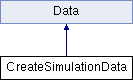
\includegraphics[width=0.2\textwidth]{class_create_simulation_data.png}
\end{figure}

\textbf{Public Member Functions}:
\begin{itemize}
\item \textbf{CreateSimulationData}(vector$<$int$>$ xCount, int sampleS): constructor, sampleS for sample size, 0 for cont., 1 for ord., 2 for nom. 
\item void \textbf{loadData}() : overload
\end{itemize}

\textbf{Private Member Functions}:
\begin{itemize}
\item void \textbf{createID}();
\item void \textbf{createActions}();
\item void \textbf{createY}();
\item void \textbf{createX}();
\item vector$<$unsigned int$>$ \textbf{createSeed}()
\item vector$<$double$>$ \textbf{createDouble}(unsigned int seed, double lowerBound = 0.0, double upperBound = 100.0)
\item vector$<$unsigned int$>$ \textbf{createInt}(unsigned int seed, unsigned int lowerBound = 0, unsigned int upperBound = 4)
\end{itemize}




More information about this class can be found from the following files:
\begin{itemize}
\item CreateSimulationData.h
\item CreateSimulationData.cpp
\end{itemize}




\subsubsection{DataInfo Class Reference}
The purpose of DataInfo class is generating the searching information for each covariant.

\begin{itemize}
\item Continuous variable:
\begin{itemize}
\item Assign cut range $\left[1,2,3,4,5,6,7,8,9,10\right]$ for available number $x \in \left\{ {0,1,2,3,4,5,6,7,8,9} \right\}$
\end{itemize}
\item Ordinal variable:
\begin{itemize}
\item Get unique value and find the corresponding cut range
\item Eg: Cut range $\left[1,2,3,4,5\right]$ for $x \in \left\{ {0,1,2,3,4} \right\}$
\end{itemize}
\item Nominal variable:
\begin{itemize}
\item Get unique value and find the corresponding cuts and cut range 
\item Eg: For $x \in \left\{ {0,1,2} \right\}$, all possible subsets are $\left\{\right\},\left\{0\right\},\left\{1\right\},\left\{2\right\},\left\{0,1\right\},\left\{0,2\right\},\left\{1,2\right\},\left\{0,1,2\right\}$. However, we only choose the short ones. As a result, inside the "nomCuts" we have $\left\{\right\},\left\{0\right\},\left\{1\right\},\left\{2\right\}$.
\end{itemize}

\end{itemize}

Flowchart of DataInfo class:
\begin{figure}[H]
\centering
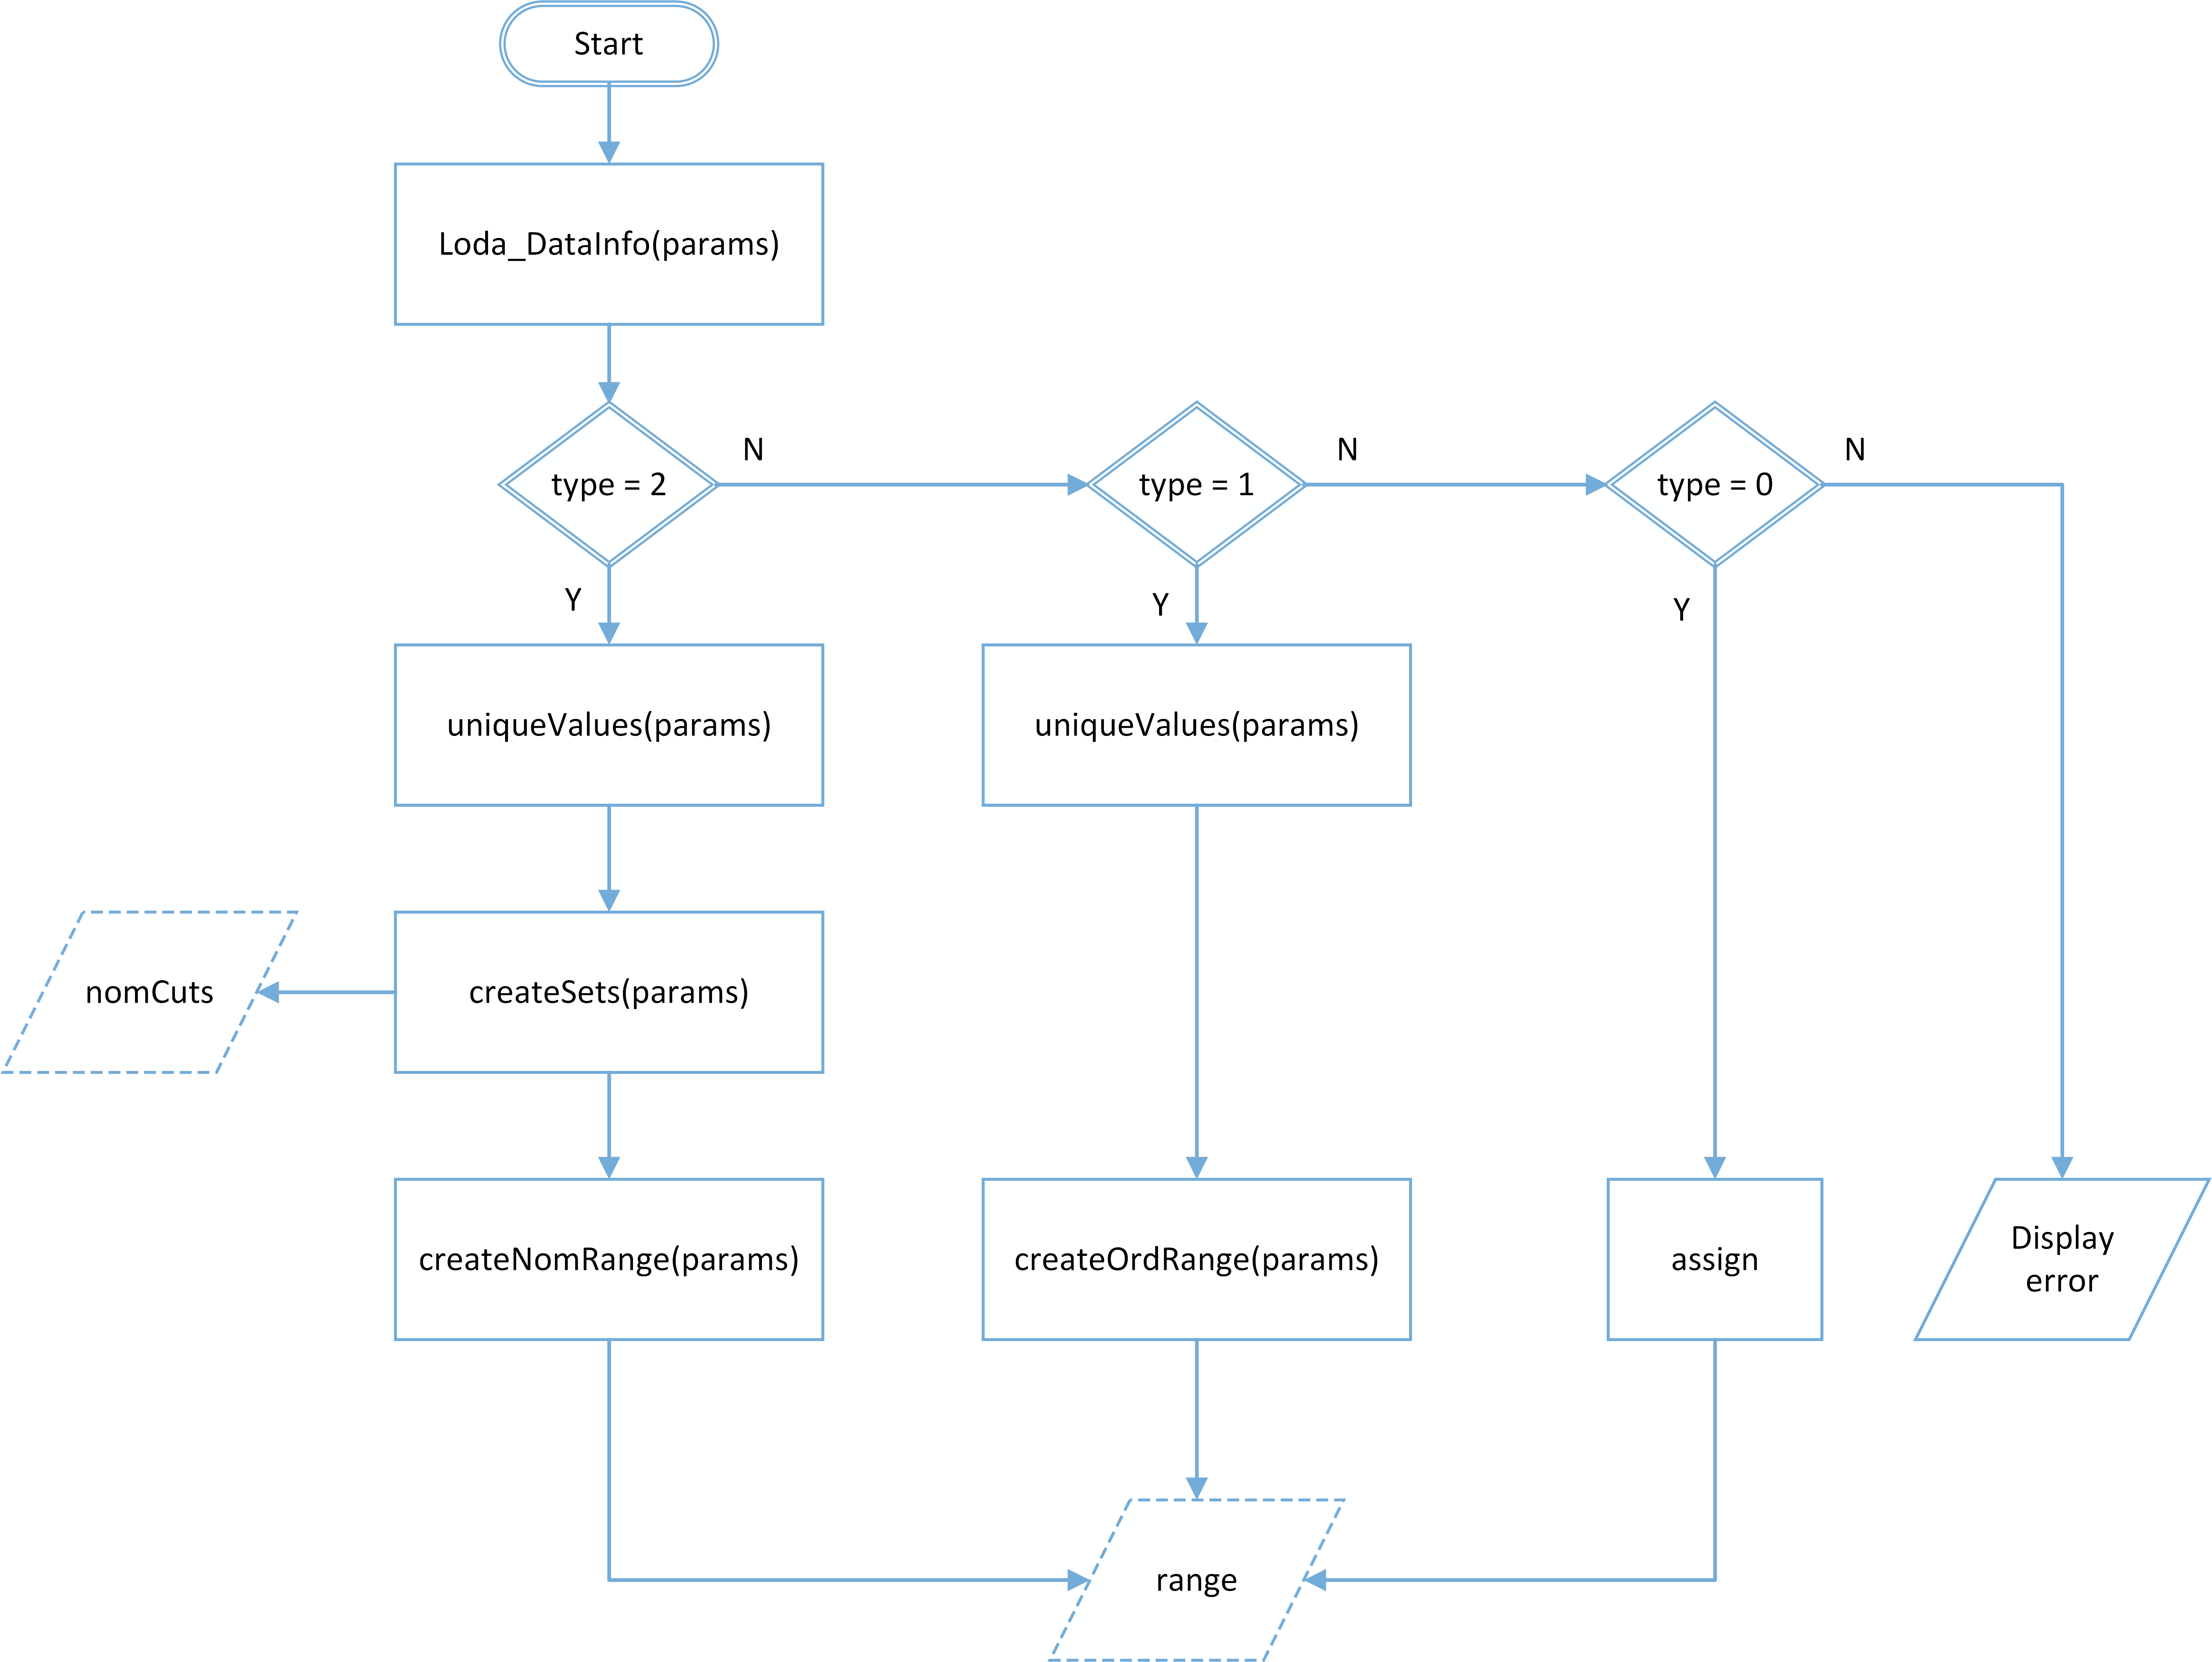
\includegraphics[width=1\textwidth]{DataInfo.png}
\end{figure}


\textbf{Private Attributes}:
\begin{itemize}
\item int varNo : variable no.
\item int varType : variable type, 0 for continuous, 1 for ordinal, 2 for nominal
\item vector$<$int$>$ range : vector for store cut range
\item vector$<$set$<$int$>>$ nomCuts : vector for store nominal cuts
\end{itemize}


\textbf{Public Member Functions}:
\begin{itemize}
\item void \textbf{load\_DataInfo} (int no, int type, vector$<$int$>$ \&dataSetColumn) : method works as constructor 
\item int \textbf{getVarNo} () : return variable no.
\item int \textbf{getVarType} () : return variable type
\item int \textbf{getCutSize} () : return no. of cuts 
\item bool \textbf{nomContains} (int x, int index) : return if nomCuts[index] contain x
\item int \textbf{getRange} (int i) : return range no. i
\item void \textbf{printVarInfo} () : print all variable info. in each object
\item void \textbf{printSet} (int i) : print set i
\end{itemize}
\textbf{Private Member Functions}
\begin{itemize}
\item vector$<$int$>$ \textbf{uniqueValues} (vector$<$int$>$ \&vectorIn)
\item vector$<$set$<$int$>>$ \textbf{createSets} (vector$<$int$>$ vectorIn)
\item vector$<$int$>$ \textbf{createNomRange} (int i) : create cut range for nominal variable
\item vector$<$int$>$ \textbf{createOrdRange} (vector$<$int$>$ x) : create cut range for percentile continuous/ordinal variable
\end{itemize}

More information about this class can be found from the following files:
\begin{itemize}
\item DataInfo.h
\item DataInfo.cpp
\end{itemize}


\subsubsection{ITR Class Reference}
The main purpose of the abstract class is store preprocessed data and implement search.

Flowchart for ITR class:
\begin{figure}[H]
\centering
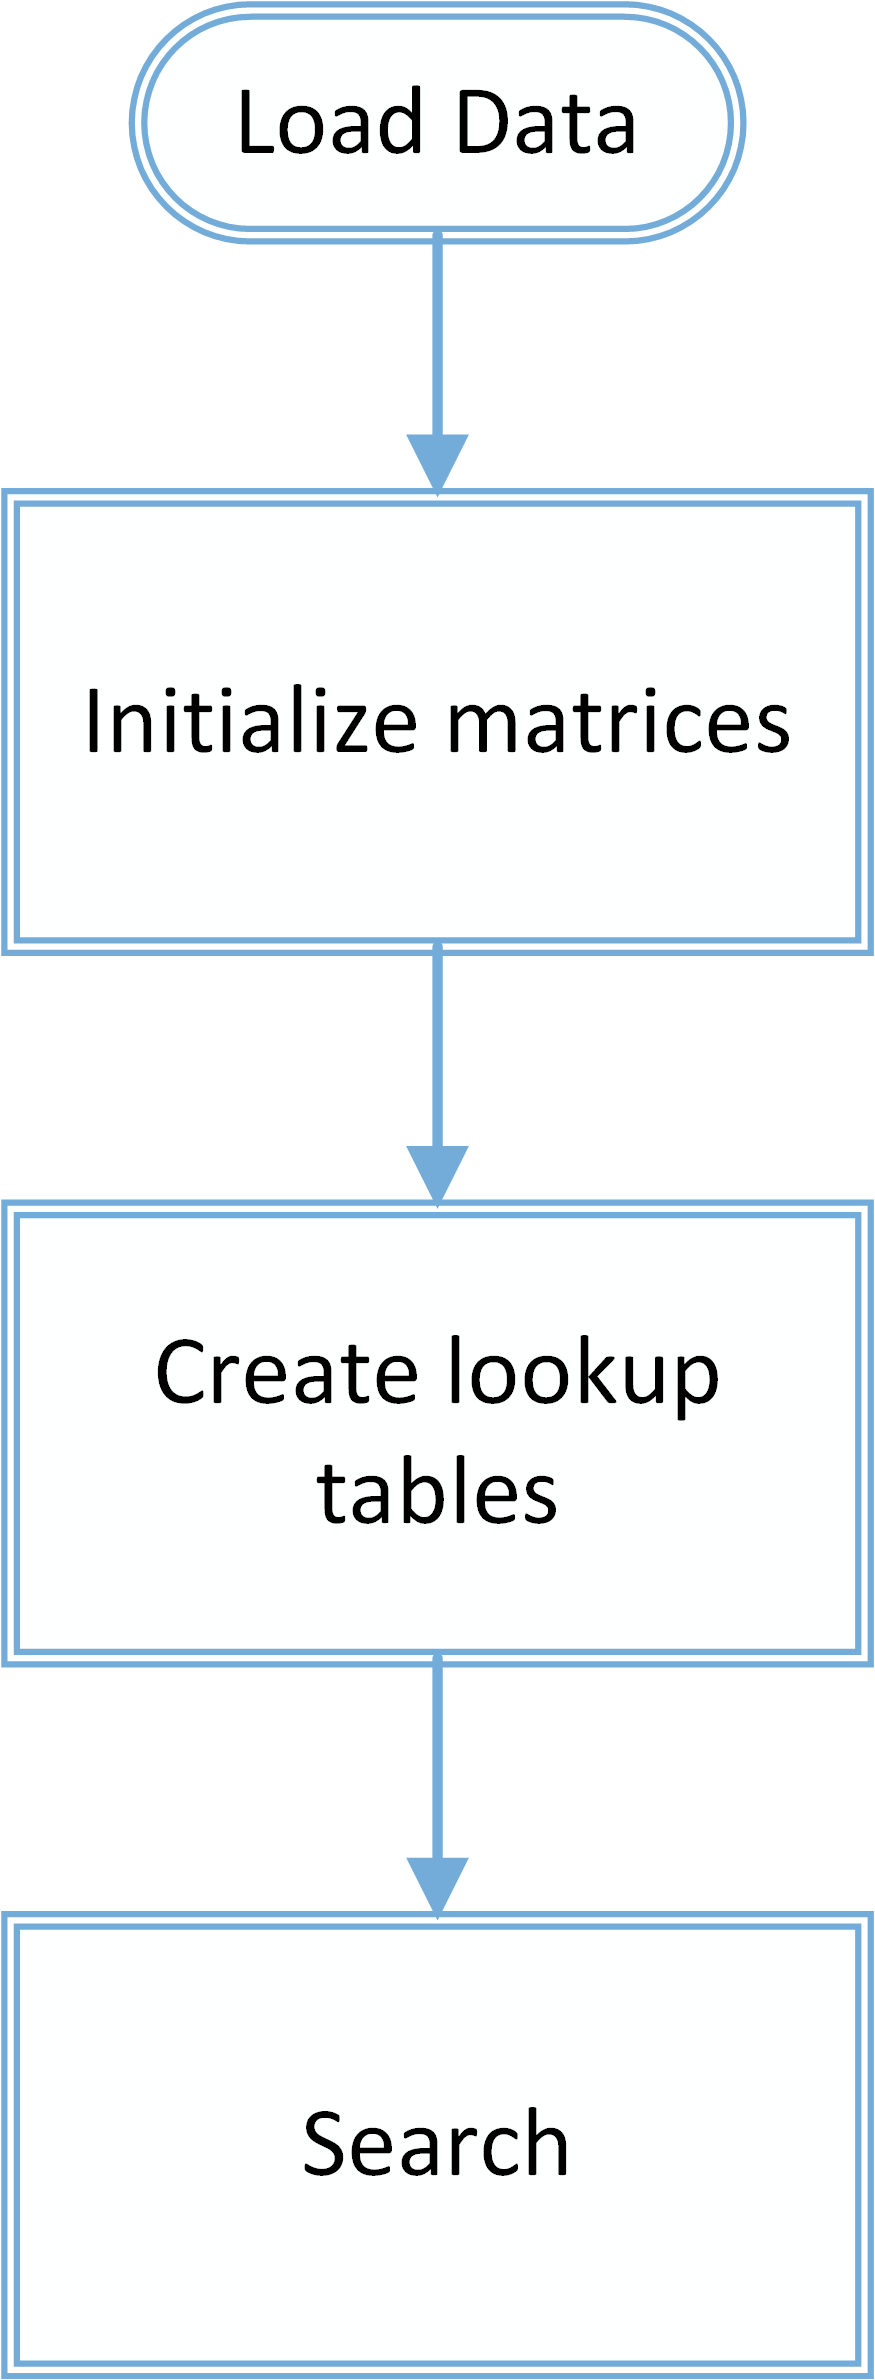
\includegraphics[width=0.20\textwidth]{ITR.png}
\end{figure}

Inheritance diagram for ITR:
\begin{figure}[H]
\centering
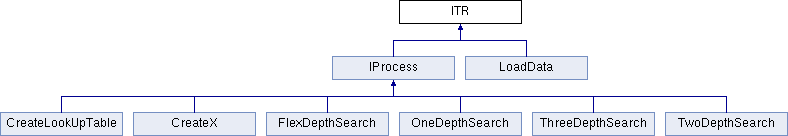
\includegraphics[width=1\textwidth]{class_i_t_r.png}
\end{figure}

\textbf{Protected Attributes}
\begin{itemize}
\item double T0 : sum of treatment 0
\item unsigned int** var\_A : 2D matrix for A  (sample\_Size $\times$ action\_Size) 
\item double** var\_Y : 2D matrix for A  (sample\_Size $\times$ y\_Size)
\item bool*** table\_X : 3D lookup table (var\_Size $\times$ cut\_Size[i] $\times$ sample\_Size) 
\item vector$<$DataInfo *$>$ info: 1D variable info. vector (var\_Size)
\item unsigned int* cut\_Size: 1D cut size vector (var\_Size)
\item static vector$<$\textbf{Res} *$>$ searchResults: vector for searching results
\end{itemize}


\textbf{Private Attributes}
\begin{itemize}
\item static Data* mydata                 
\item static vector$<$unsigned int$>$ var\_Type   
\item static vector$<$vector$<$unsigned int$>>$ var\_X
\end{itemize}



\textbf{Public Member Functions}
\begin{itemize}
\item \textbf{ITR} (): constructor
\item virtual void \textbf{process} ()  
\item static void \textbf{setData}(\textbf{Data}* data)                  
\item static void \textbf{setVarType}(vector$<$unsigned int$>$ X)          
\item static void \textbf{setX}(vector$<$vector$<$unsigned int$>>$ X)       
\item static \textbf{Data}* \textbf{getData}();                      
\item static vector$<$vector$<$unsigned int$>>$\& \textbf{getX}(); 
\item static double \textbf{getT0}();                       
\item static vector$<$unsigned int$>$ \textbf{getVarType}();    
\item static vector$<$\textbf{Res} *$>$ \textbf{getSearchResults}(); 
\end{itemize}







More information about this class can be found from the following files:
\begin{itemize}
\item ITR.h
\item ITR.cpp
\end{itemize}


\subsubsection{LoadData Class Reference}
The purpose of LoadData class is for load data

Inheritance diagram for LoadData:
\begin{figure}[H]
\centering
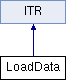
\includegraphics[width=0.2\textwidth]{class_load_data.png}
\end{figure}

\textbf{Private Attributes}:
\begin{itemize}
\item \textbf{Data}* m\_data
\end{itemize}

\textbf{Public Member Functions}
\begin{itemize}
\item \textbf{LoadData } (\textbf{Data} *data) : constructor
\item void \textbf{process} () : overload
\end{itemize}

More information about this class can be found from the following files:
\begin{itemize}
\item LoadData.h
\item LoadData.cpp
\end{itemize}


\subsubsection{IProcess Class Reference}
IProcess is an abstract class for processing data.

Inheritance diagram for IProcess:
\begin{figure}[H]
\centering
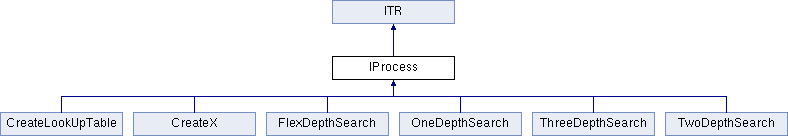
\includegraphics[width=1\textwidth]{class_i_process.png}
\end{figure}

\textbf{Protected Attributes}:
\begin{itemize}
\item \textbf{ITR}* myITR
\end{itemize}

\textbf{Public Member Functions}
\begin{itemize}
\item \textbf{IProcess} (\textbf{ITR} *itr) : constructor
\item virtual void \textbf{process} () : virtual function
\end{itemize}

More information about this class can be found from the following files:
\begin{itemize}
\item IProcess.h
\item IProcess.cpp
\end{itemize}



\subsubsection{CreateX  Class Reference}
The purpose of CreateX class is for preprocessing data
\begin{itemize}
\item Convert double to unsigned int
\item Combine variables
\end{itemize}

Inheritance diagram for CreateX:
\begin{figure}[H]
\centering
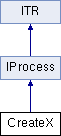
\includegraphics[width=0.2\textwidth]{class_create_x.png}
\end{figure}

\textbf{Public Member Functions}
\begin{itemize}
\item \textbf{CreateX} (\textbf{ITR} *itr) : constructor
\item void \textbf{process} () : overload
\end{itemize}

\textbf{Private Member Functions}
\begin{itemize}
\item vector$<$vector$<$unsigned int$>>$ \textbf{percentileVec}(vector$<$vector$<$double$>>$ const \&vectIn);
\item vector$<$unsigned int$>$ \textbf{percentileVec}(vector$<$double$>$ const \&vectIn);
\item std::map$<$double, unsigned int$>$ \textbf{percentileMap}(vector$<$double$>$ const \&vectorIn);
\item double \textbf{percentile}(double len,double index);
\item unsigned int \textbf{assignPercentile}(double p);
\item vector$<$vector$<$unsigned int$>>$ \textbf{combineData}();
\end{itemize}

More information about this class can be found from the following files:
\begin{itemize}
\item CreateX.h
\item CreateX.cpp
\end{itemize}


\subsubsection{CreateLookUpTable Class Reference}
The purpose of CreateLookUpTable class is for create lookup table.

Inheritance diagram for CreateLookUpTable:
\begin{figure}[H]
\centering
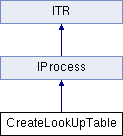
\includegraphics[width=0.25\textwidth]{class_create_look_up_table.png}
\end{figure}

\textbf{Private Attributes}:
\begin{itemize}
\item unsigned int actionIndex;
\item unsigned int sampleSize;
\item unsigned int varSize;
\item unsigned int actionSize;
\item unsigned int ySize;
\end{itemize}

\textbf{Public Member Functions}
\begin{itemize}
\item \textbf{CreateLookUpTable} (\textbf{ITR} *itr, unsigned int index=0) : constructor, index for select 0 action
\item void \textbf{process} () : overload
\end{itemize}

\textbf{Private Member Functions}
\begin{itemize}
\item void init() : initial dynamic allocation
\item void load\_CutSize() : load cut size
\item void init\_TableX()
\item void load\_table\_X(const vector$<$vector$<$unsigned int$>>$ \&data\_X)
\item void load\_Action(const vector$<$vector$<$unsigned int$>>$ \&data\_A)
\item void load\_Y(const vector$<$vector$<$double$>>$ \&data\_Y)
\item void cleanAll() : delete dynamic allocation
\item double sumTreatmentCal() : sum Y given A = index
\end{itemize}

More information about this class can be found from the following files:
\begin{itemize}
\item CreateLookUpTable.h
\item CreateLookUpTable.cpp
\end{itemize}

\subsubsection{ThreeDepthSearch Class Reference}
The purpose of ThreeDepthSearch class is for 3 depth comprehensive search.

Flowchart for ThreeDepthSearch class:
\begin{figure}[H]
\centering
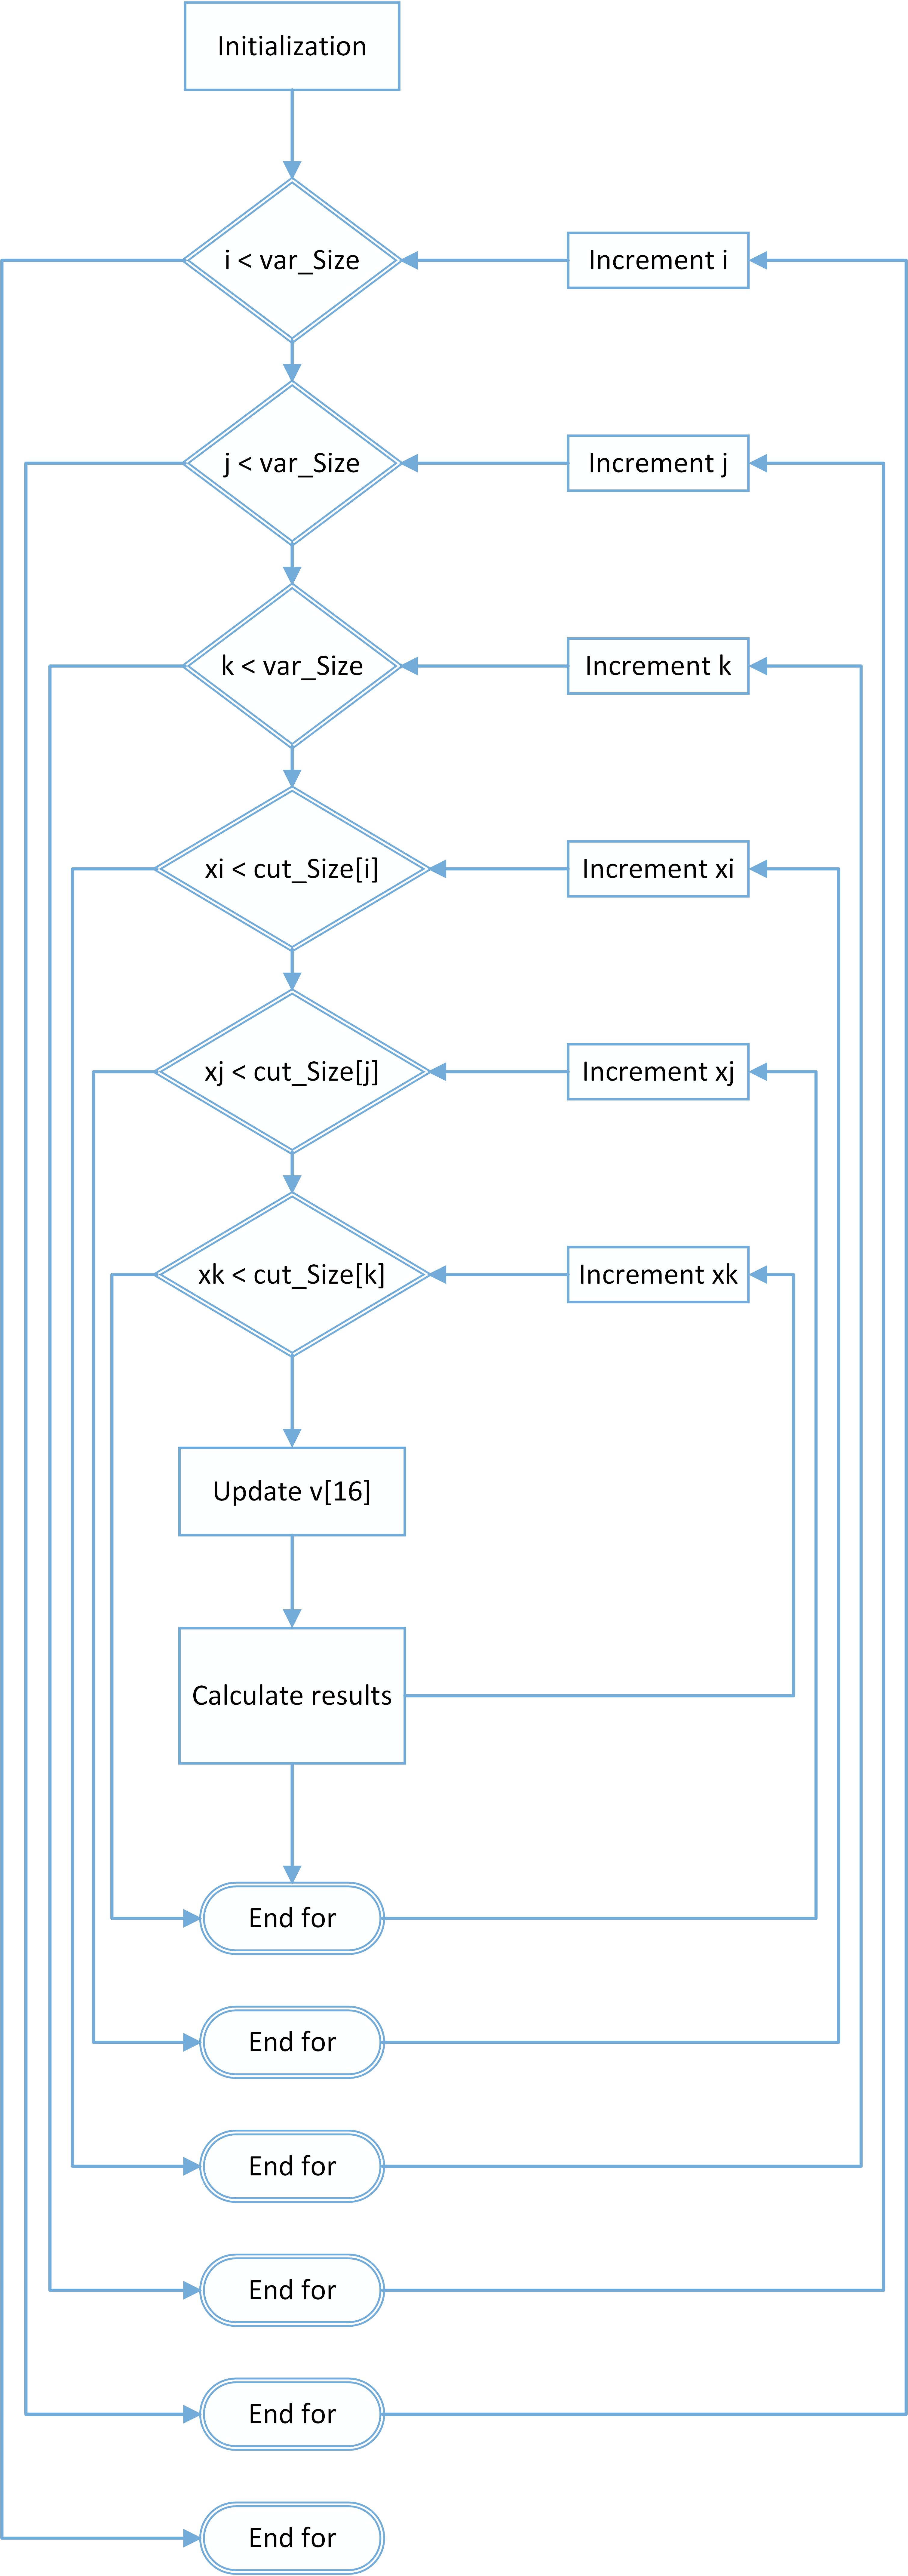
\includegraphics[width=0.5\textwidth]{ThreeDepth.png}
\end{figure}

Inheritance diagram for ThreeDepthSearch:
\begin{figure}[H]
\centering
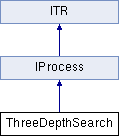
\includegraphics[width=0.25\textwidth]{class_three_depth_search.png}
\end{figure}

\textbf{Private Attributes}:
\begin{itemize}
\item unsigned int depth;                
\item bool isPrint;                      
\item unsigned int sampleSize;           
\item unsigned int varSize;                 
\end{itemize}

\textbf{Public Member Functions}
\begin{itemize}
\item \textbf{ThreeDepthSearch} (\textbf{ITR}* itr, bool print = true) : constructor
\item void \textbf{process} () :  override function
\end{itemize}

\textbf{Private Member Functions}
\begin{itemize}    
\item void \textbf{searchPrint}() : print results
\item vector$<$\textbf{Res} *$>$ \textbf{searchOutput}() : output results
\end{itemize}

More information about this class can be found from the following files:
\begin{itemize}
\item ThreeDepthSearch.h
\item ThreeDepthSearch.cpp
\end{itemize}



\subsubsection{FlexDepthSearch Class Reference}
The purpose of FlexDepthSearch class is for flexible depth comprehensive search. It is mainly comprised of three loops: 
\begin{itemize}
\item Outer loop: loop through all variable combinations
\item Middle loop: loop through all possible cuts for given variable(s)
\item Inner loop: loop through samples for searching 
\end{itemize}

Flowchart for FlexDepthSearch class:
\begin{figure}[H]
\centering
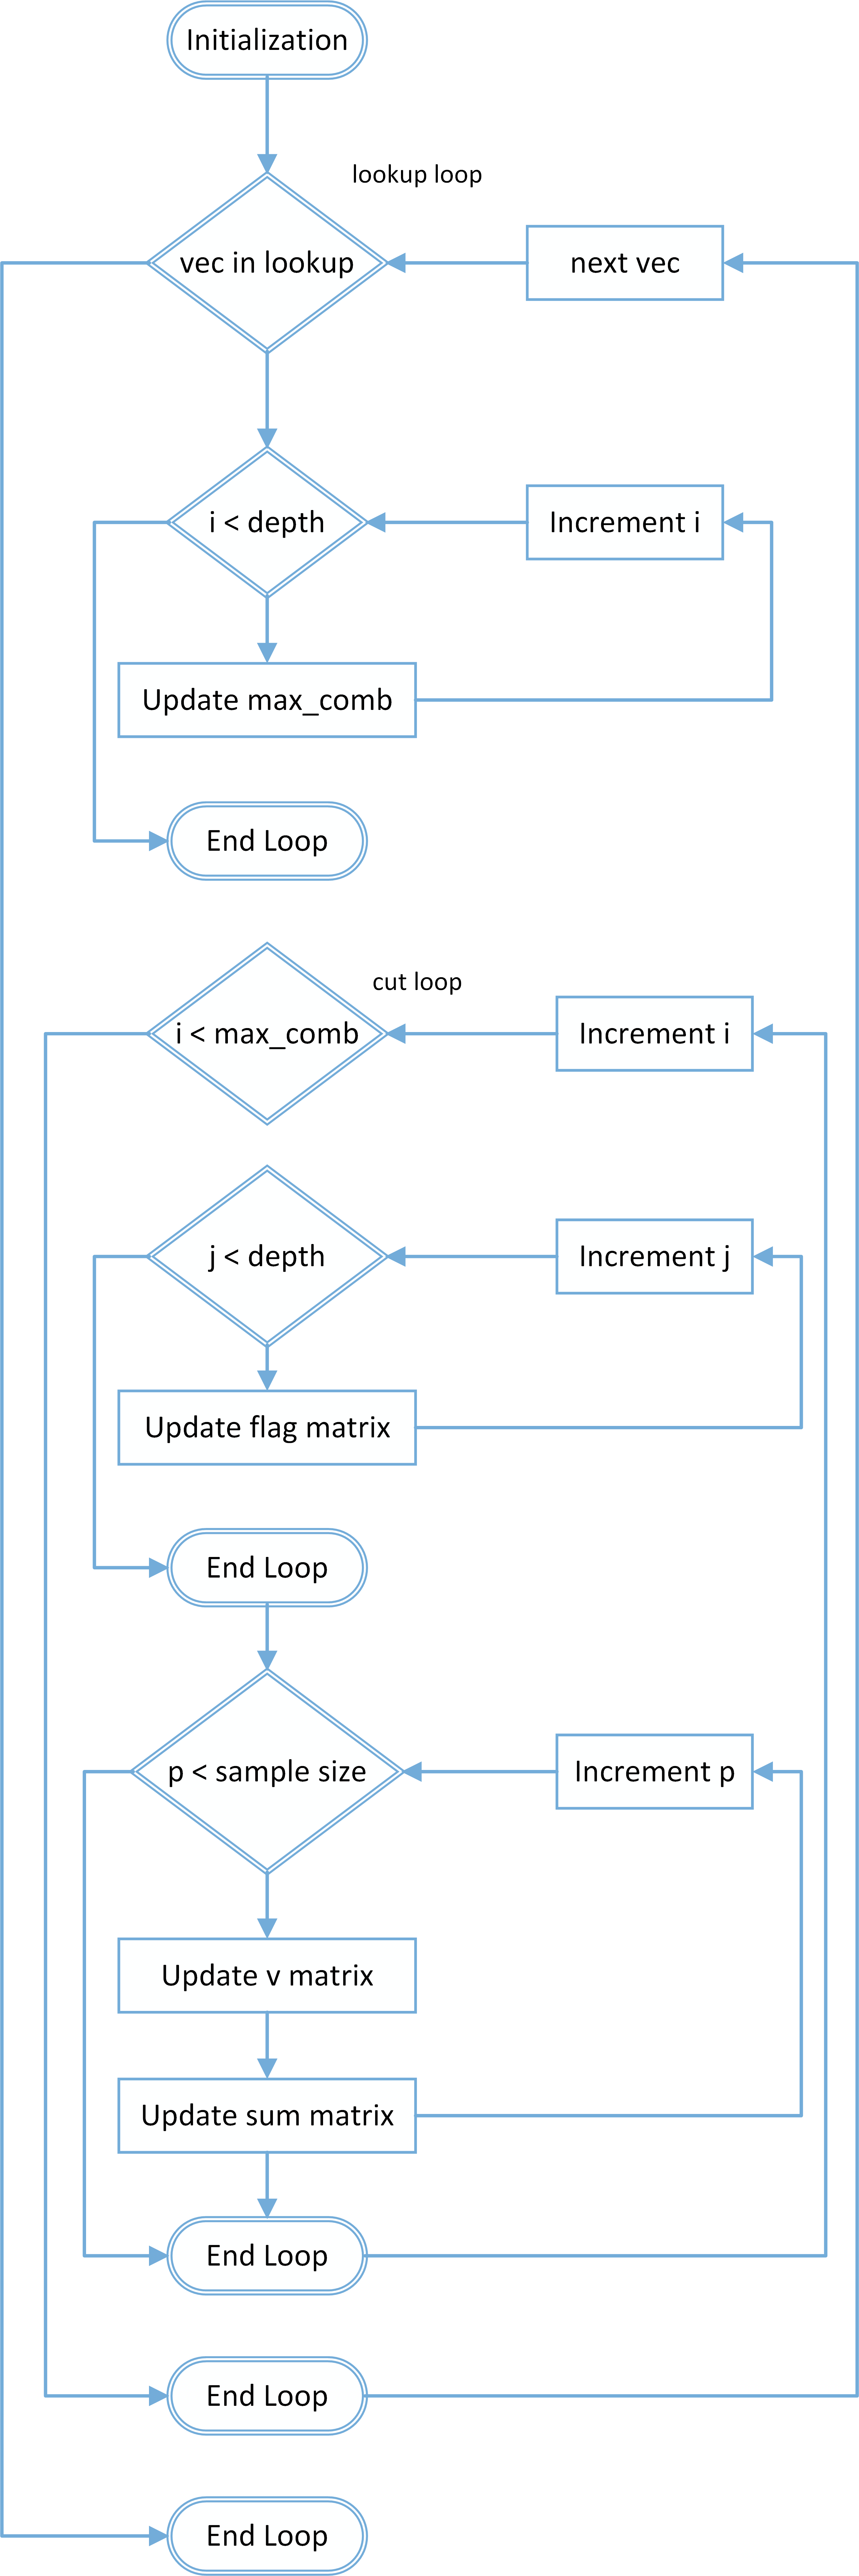
\includegraphics[width=0.5\textwidth]{FlexDepth.png}
\end{figure}

Inheritance diagram for FlexDepthSearch:
\begin{figure}[H]
\centering
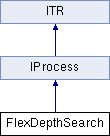
\includegraphics[width=0.25\textwidth]{class_flex_depth_search.png}
\end{figure}

\textbf{Private Attributes}:
\begin{itemize}
\item unsigned int depth;                
\item bool isPrint;                      
\item unsigned int sampleSize;           
\item unsigned int varSize;              
\item vector$<$unsigned int$>$ varType;
\item vector$<$vector$<$int$>>$ lookup;    
\end{itemize}

\textbf{Public Member Functions}
\begin{itemize}
\item \textbf{FlexDepthSearch} (\textbf{ITR}* itr, unsigned int d, bool print = true) : constructor, d for search depth
\item void \textbf{process} () :  override function
\end{itemize}

\textbf{Private Member Functions}
\begin{itemize}    
\item vector$<$vector$<$int$>>$ \textbf{combine}(int n, int k) : create lookup for outer loop
\item void \textbf{searchPrint}() : print results
\item vector$<$\textbf{Res} *$>$ \textbf{searchOutput}() : output results
\end{itemize}


More information about this class can be found from the following files:
\begin{itemize}
\item FlexDepthSearch.h
\item FlexDepthSearch.cpp
\end{itemize}


\subsubsection{Res Class Reference}
\textbf{Private Attributes}:
\begin{itemize}
\item float result: results
\item vector$<$int$>$* index: variable combination information
\item int direction: cut direction information
\end{itemize}


\textbf{Public Member Functions}
\begin{itemize}
\item \textbf{Res} (double res, vector$<$unsigned int$>$ ind, int dir): construction
\item float \textbf{getRes} (): return result
\item vector$<$unsigned int$>$ \textbf{getIndex} $\left(\right)$: return variable combination
\begin{itemize}
\item Eg: 1 depth search: \{1 2\} means var 1 with cut 2
\item Eg: 2 depth search: \{1 2 3 4\} means var 1 with cut 2, var 3 with cut 4
\end{itemize}

\item int \textbf{getDirection} (): return cut directions
\begin{itemize}
\item Eg: 1 depth search: 1 means satisfy criteria, 0 means not satisfy criteria
\item Eg: 2 depth search: 0 means not satisfy criteria 1 and 2, 1 means satisfy criteria 2 but not satisfy criteria 1, 2 means satisfy 1 but not satisfy criteria 2, 3 means satisfy criteria 1 and 2 
\end{itemize}

\end{itemize}

More information about this class can be found from the following files:
\begin{itemize}
\item Res.h 
\item Res.cpp
\end{itemize}



\pagebreak
\section{Test}
In this simulation, we proposed 3000 samples, each with total 35 variables. The 35 variables are comprised of 25 continuous variables, 5 ordinal variables (range 0 to 4), and 5 nominal variables (range 0 to 4). A binary treatment is assigned uniformly for each patient. The response is assigned randomly to the range of 0 to 100. 


\subsection{System information}
\begin{itemize}
\item System Type:
System Type	x64-based PC
\item Processor: 
Processor	Intel(R) Core(TM) i5-6300U CPU @ 2.40GHz, 2401 Mhz, 2 Core(s), 4 Logical Processor(s)
\item Installed Physical Memory (RAM):	8.00 GB
\end{itemize}


\subsection{Run-time performance test}
\begin{itemize}
\item Fixed step search (ThreeDepthSearch)
\begin{itemize}
\item Print: around 60s
\item Output: around 50s 
\end{itemize}
\item Flexible step search (FlexDepthSearch) with depth  = 3
\begin{itemize}
\item Print: around 90s
\item Output: around 75s 
\end{itemize}
\end{itemize}


\subsection{Unit testing}
For unit testing "googletest" is implemented by using Microsoft Visual Studio. Python is employed for result validation.

Three test datasets have been used for testing.
\begin{itemize}
\item Simple test data (1 ord)
\item CSV test data (3 cont, 3 ord, 3 nom)
\item Simulated test data (2 cont, 3 ord, 4 nom)
\end{itemize}

30 tests for 8 test cases haven been run for testing.


Store 100 samples, 9 variables(3 continuous variables, 3 continuous variables, 3 nominal variables)
\begin{enumerate}
\item DataInputTest
\begin{enumerate}
\item[1.1] TestSimpleInputData: validate input data for simple test data
\item[1.2] TestReadCSV\_Size: validate data size for CSV test data
\item[1.3] TestReadCSV\_Value: validate input data for CSV test data
\item[1.4] TestSimulationData\_Size: validate data size for simulated data
\end{enumerate}
\item LoadDataTest
\begin{enumerate}
\item[2.1] SimpleTestData: validate "class LoadData" for simple test data
\item[2.2] CSVData: validate "class LoadData" for CSV test data
\item[2.3] SimulationData: validate "class LoadData" for simulated data
\end{enumerate}
\item CreateXTest
\begin{enumerate}
\item[3.1] SimpleTestData: validate "class CreateX" for simple test data
\item[3.2] CSVTestData: validate "class CreateX" for CSV test data
\item[3.3] SimulationData: validate "class CreateX" for simulated data
\end{enumerate}
\item CreateLookUpTableTestTest
\begin{enumerate}
\item[4.1] SimpleTestData\_Part\_I: validate DataInfo for "class CreateLookUpTable" with simple test data
\item[4.2] SimpleTestData\_Part\_II: validate lookup table for "class CreateLookUpTable" with simple test data
\item[4.3] CSVData\_Part\_I: validate DataInfo for "class CreateLookUpTable" with CSV test data
\item[4.4] CSVData\_Part\_II: validate lookup table for "class CreateLookUpTable" with CSV test data
\item[4.5] SimulatedData: validate DataInfo for "class CreateLookUpTable" with simulated data
\end{enumerate}
\item OneDepthSearchTest
\begin{enumerate}
\item[5.1] SimpleTestData\_Part\_I: validate "class OneDepthSearch" for print with simple test data
\item[5.2] SimpleTestData\_Part\_II: validate "class OneDepthSearch" for output with simple test data
\item[5.3] CSVData\_Part\_I: validate "class OneDepthSearch" for print with CSV test data
\item[5.4] CSVData\_Part\_II: validate "class OneDepthSearch" for output with CSV test data
\item[5.5] SimulationTestData: validate "class OneDepthSearch" for output with simulated data
\end{enumerate}
\item TwoDepthSearchTest
\begin{itemize}
\item[6.1] CSVTestData: validate "class TwoDepthSearch" for output with CSV test data
\item[6.2] SimulationTestData: validate "class TwoDepthSearch" for output with simulated data
\end{itemize}
\item ThreeDepthSearchTest
\begin{itemize}
\item[7.1] CSVTestData: validate "class ThreeDepthSearch" for output with CSV test data
\item[7.2] SimulationTestData: validate "class ThreeDepthSearch" for output with simulated data
\end{itemize}
\item FlexDepthSearchTest
\begin{enumerate}
\item[8.1] CSVTestData\_1D: validate "class FlexDepthSearch" for depth 1 with CSV data
\item[8.2] CSVTestData\_2D: validate "class FlexDepthSearch" for depth 2 with CSV data
\item[8.3] CSVTestData\_3D: validate "class FlexDepthSearch" for depth 3 with CSV data
\item[8.4] SimulatedTestData\_1D: validate "class FlexDepthSearch" for depth 1 with simulated data
\item[8.5] SimulatedTestData\_2D: validate "class FlexDepthSearch" for depth 2 with simulated data
\item[8.6] SimulatedTestData\_3D: validate "class FlexDepthSearch" for depth 3 with simulated data
\end{enumerate}


\end{enumerate}


























\pagebreak
\section{Future work}
\begin{enumerate}
\item Add more recommendation algorithms 
\item Add more data preprocessing methods, eg. data cleaning method
\end{enumerate}


\include{bibliography}






\end{document}

